\chapter{Experimental Evaluation}
\label{chap:experimental_evaluation}

In this chapter we first describe the datasets on which we conducted the experiments, and establish an objective explanation quality measure. We then present and analyze a few results of our approximate lineage system.


\section{Experimental Setup}\label{sec:evaluation-setup}
We used two datasets from different domains (food and movies) to compare the performance of our approximate lineage system against ProvSQL. The goal of these experiments is evaluating the precision of our approximate explanations against an ``exact provenance tracking system".
\par\textbf{Note.} \textit{max\_vectors\_num} (see section \ref{sec:proposed_solution_approx}) was chosen manually to be 4. The optimization of hyperparameters, and, specifically, \textit{max\_vectors\_num} - is the subject of ongoing research.\\

% USDA BFPD and MovieLens
\subsection{Datasets}\label{sec:datasets}
\begin{enumerate}
    \item The USDA Branded Food Products Database (BFPDB) \cite{usda_bfpd-dataset} is the result of a Public-Private Partnership, whose goal is to enhance public health and the sharing of open data by complementing USDA Food Composition Databases with nutrient composition of branded foods and private label data, provided by the food industry. Among others, the dataset includes three tables:
    \begin{itemize}
        \item \texttt{products} - contains basic information on branded products (manufacturer, name, ingredients).
        \item \texttt{serving\_size} - each tuple contains information about a product's serving size (as well as unit of measure) and food preparation state.
        \item \texttt{nutrients} - each tuple contains all nutrient value information about a product.
    \end{itemize}
    Each product in the BFPDB dataset has a unique identifier, \texttt{ndb\_no}.
    
    \item The MovieLens dataset \cite{movielens-dataset} describes people’s preferences for movies. These preferences are entered by way of the MovieLens website \cite{movielens-recommender-website} — a recommender system that asks its users to provide movie ratings in order to receive personalized movie recommendations. Among others, the dataset includes three tables:
    \begin{itemize}
        \item \texttt{movies} - each tuple contains basic information about a movie (title, genres).
        \item \texttt{ratings} - each tuple contains information about a user's expressed preference of a movie (a 0-5 star rating).
        \item \texttt{tags} - each tuple contains information about a user's classifying tag of a movie (silly, funny, etc.).
    \end{itemize}
    Each movie in the MovieLens dataset has a unique identifier, \texttt{movieId}.
\end{enumerate}

% Explain how the precision evaluation process works (test against lineage from provsql)
\subsection{Precision Calculation}\label{sec:precision}
In section \ref{sec:proposed_solution_approx} we stated that we expect our explanations to approximate the exact lineage of query result tuples. 
Thus, in order to test the aforementioned algorithms and implementation, we devised an explanation quality measure for explaining a single tuple $t$: 
\begin{equation*}
    \operatorname{Precision}(t, n) = \frac{|ApproxLineage(t, n) \cap ExactLineage(t)|}{|ApproxLineage(t, n)|}\\
\end{equation*}
where $ApproxLineage(t, n)$ is the set of the top $n$ (by lineage similarity) tuples, returned as explanations (i.e., approximate lineage) for $t$ by our system. $ExactLineage(t)$ is the set of tuples that comprise the exact \textbf{distant} lineage of $t$, calculated recursively from the semiring polynomial that is returned by the ProvSQL system.
For example, if the direct lineage of $t_4$ and $t_5$ are the sets $\{t_1, t_2, t_3\}$ and $\{t_1\}$, respectively, and the direct lineage of a tuple $t_6$ is the set $\{t_4, t_5\}$ then the total distant lineage for the tuple $t_6$ is $\{t_1, t_2, t_3, t_4, t_5\}$.
The parameter $n$ is set by us in each experiment, that is, it is a parameter of the experiment. 
Observe that $\operatorname{Precision(t, n)}$ is tunable via the parameter $n$, i.e., when $n$ is small we test for precision of the ``top" explanations we found.\\
\par Classically, we are usually interested in precision and recall (e.g., in traditional statistics and classification problems). However, here the situation is slightly different, what we really are interested in is to assess the quality of our explanations by measuring ``how many of the top $n$ (by lineage similarity) tuples are actually part of the exact lineage?". By contrast, traditional recall does not seem to be a meaningful metric in our case, as many query-result tuples might have long histories. Hence, a top-N justifications result is preferred over ``returning all the correct lineage tuples", and this is what we measure.

\subsection{Distant Lineage: Per-Level Recall}\label{sec:recall}
    In order to assess the quality of a distant lineage answer in a more insightful way, we save the ``exact distant lineage" in a hierarchical structure, and analyze it per-level. One possible implementation is a list $L$ of sets per-tuple, s.t. $L[i]$ is the set of all lineage tuples at the $i^{th}$ derivation depth level. Note that $i$ starts at $0$, s.t. the $0^{th}$ lineage level is a set containing the target tuple only. For example, if the direct lineage of $t_4$ and $t_5$ are the sets $\{t_1, t_2, t_3\}$ and $\{t_1\}$, respectively, and the direct lineage of a tuple $t_6$ is the set $\{t_3, t_4, t_5\}$ (note that $t_3$ appears in both the $1^{st}$ and the $2^{nd}$ lineage levels of $t_6$, in this example) then the hierarchical lineage tree for the tuple $t_6$, and the hierarchical list structure that represents it, look as follows: \\\\
    % A simple Tree
% Author: Stefan Kottwitz
% https://www.packtpub.com/hardware-and-creative/latex-cookbook
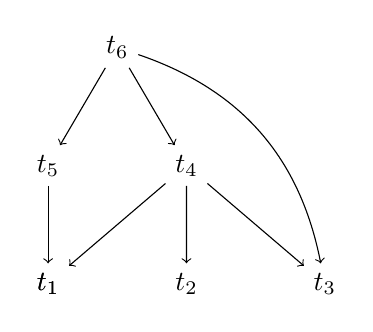
\begin{tikzpicture}[sibling distance=5em,
  edge from parent/.style={->,draw},
  every edge/.style={->,draw}
  ]]
  \node(t_6) {$t_6$}
    child { node {$t_5$} 
      child { node {$t_1$} } 
      }
    child { node {$t_4$}
      child { node {$t_1$} }
      child { node {$t_2$} }
      child { node(t_3) {$t_3$} }
      };
      
    \draw (t_6) edge[bend left] (t_3);
\end{tikzpicture} \hspace{35pt}
    % A simple Tree
% Author: Stefan Kottwitz
% https://www.packtpub.com/hardware-and-creative/latex-cookbook
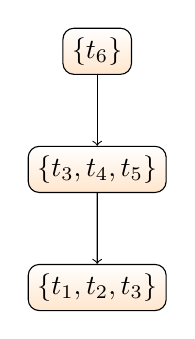
\begin{tikzpicture}[sibling distance=3em,
  every node/.style = {shape=rectangle, rounded corners,
    draw, align=center,
    top color=white, bottom color=orange!20},
  edge from parent/.style={->,draw}
  ]]
  \node {$\{t_6\}$}
    child { node {$\{t_3, t_4, t_5\}$} 
      child { node {$\{t_1, t_2, t_3\}$} } 
      };
\end{tikzpicture} \\\\
Here, each rectangle is an entry in the list $L$.
\par We expect our explanations to have a ``natural ranking" property in terms of lineage levels. That is, we expect the similarity between a target tuple and tuples in its distant lineage to be inversely proportional to the distance between them in the hierarchical lineage tree structure. Thus, we devise an explanation quality measure for the explanation of a single tuple $t$ and its lineage level $i$:
\begin{equation*}
    \operatorname{Recall}(t, i) = \frac{|ApproxLineage(t, D(t, i)) \cap L_t[i])|}{|L_t[i]|}\\
\end{equation*}
where $ApproxLineage(t, D(t, i))$ is the set of the top $D(t, i)$ (by lineage similarity) tuples, returned as explanations (i.e., approximate lineage) for $t$ by our system.
$D(t, i)$ is the number of unique returned tuples in the lineage of $t$ up until the $i^{th}$ level (including). Formally, it is defined as follows: $D(t, i) = |\bigcup\limits_{j=1}^{i} L_t[j]|$.
$L_t$ is the hierarchical list structure for $t$, as defined above, s.t. $L_t[i]$ is the set of all lineage tuples at the $i^{th}$ derivation depth level of $t$.\\

\section{Examples}

Having established an objective explanation quality measure, we conducted a series of experiments. In particular, we tested the precision on direct provenance of different queries, varying from ``simple" (examples \ref{experiment:1} and \ref{experiment:2}) to ``complex" (example \ref{experiment:3}) queries. We show some of the experimental results and present a qualitative analysis.
\par\textbf{Note.} In all the examples, the lineage (and its size - `Lin. size' column) of a tuple, is calculated as a subset of the exact lineage. That is, if we compare a query result tuple with all the tuples in the \texttt{products} table (in order to find the top $N$ most similar tuples) - we use only \texttt{product} tuples in the exact lineage for precision calculations ($Lineage\_products(t)$ = $ExactLineage(t) \cap \texttt{products}.tuples$).


\begin{runexample}
We test queries on a small subset of the MovieLens dataset. Each table (i.e., \texttt{movies}, \texttt{ratings}, \texttt{tags}) consists of about 10,000 tuples.
\end{runexample}
%%% Present here all the queries? Figure? I think NO

% Example 1
% MovieLens tuples vs. columns.
% \begin{table}
\centering
% \begin{adjustbox}{width=\columnwidth,center}
\pgfplotstabletypeset[
    color cells={min=0.45,max=1.0}, format index, format table, format userId,
    col sep=comma,
    /pgfplots/colormap={orange}{
        rgb255(0cm)=(255,245,235);
        rgb255(1cm)=(253,141,60)},
    assign column name/.code=\pgfkeyssetvalue{/pgfplots/table/column
        name}{{\textbf{#1}}},
]{
    % index,     userId, {lineage size},  {tuple$_{all}$}, {tuple$_{half}$}, {cols$_{all}$}, {cols$_{half}$}                      
    % 0,     275402,            3,          0.667 ,        1.0 ,            1.0 ,           1.0
    % 1,     275707,            1,          1.000 ,        1.0 ,            1.0 ,           1.0
    % 2,     275980,            1,          1.000 ,        1.0 ,            1.0 ,           1.0
    % 3,     278069,            1,          0.845 ,        1.0 ,            0.92 ,           1.0
    % 4,     279177,            1,          1.000 ,        1.0 ,            1.0 ,           1.0
    % 5,     280810,            1,          1.000 ,        1.0 ,            1.0 ,           1.0
    % 6,     282342,            3,          0.667 ,        1.0 ,            1.0 ,           1.0
    % 7,     282405,            2,          1.000 ,        1.0 ,            1.0 ,           1.0
    
    index,     userId, {Lin. size},  {Precision$^{tuples}$},  {Precision$^{cols}$}                 
    0,     275402,            3,          0.667 ,                  1.0  
    1,     275707,            1,          1.000 ,                  1.0  
    2,     275980,            1,          1.000 ,                  1.0  
    3,     278069,            1,          1.000 ,                  1.0     
    4,     279177,            1,          1.000 ,                  1.0  
    5,     280810,            1,          1.000 ,                  1.0  
    6,     282342,            3,          0.667 ,                  1.0  
    7,     282405,            2,          1.000 ,                  1.0  

}
% \end{adjustbox}
\textbf{\caption{\label{tab:1}
                \texttt{userId} indicates the unique user's identifier returned by the query. Lin. size is the size of the exact lineage for a result tuple (containing only tuples from the \texttt{tags} table). Precision$^{tuples}$ and Precision$^{cols}$ display our system's precision for each tuple in the result, for both ``lineage tuple vectors" and ``lineage column vectors" (with query-specific column weighting), respectively. Precision computations are done for the top $n = |Lineage\_tags(t)\protect\footnotemark|$ tuples in the approximate lineage for each result tuple $t$.
                }
        }
\end{table}
% "Toy" example
\begin{example-withrun}\label{experiment:1}
\begin{table}
\centering
% \begin{adjustbox}{width=\columnwidth,center}
\pgfplotstabletypeset[
    color cells={min=0.45,max=1.0}, format index, format table, format userId,
    col sep=comma,
    /pgfplots/colormap={orange}{
        rgb255(0cm)=(255,245,235);
        rgb255(1cm)=(253,141,60)},
    assign column name/.code=\pgfkeyssetvalue{/pgfplots/table/column
        name}{{\textbf{#1}}},
]{
    % index,     userId, {lineage size},  {tuple$_{all}$}, {tuple$_{half}$}, {cols$_{all}$}, {cols$_{half}$}                      
    % 0,     275402,            3,          0.667 ,        1.0 ,            1.0 ,           1.0
    % 1,     275707,            1,          1.000 ,        1.0 ,            1.0 ,           1.0
    % 2,     275980,            1,          1.000 ,        1.0 ,            1.0 ,           1.0
    % 3,     278069,            1,          0.845 ,        1.0 ,            0.92 ,           1.0
    % 4,     279177,            1,          1.000 ,        1.0 ,            1.0 ,           1.0
    % 5,     280810,            1,          1.000 ,        1.0 ,            1.0 ,           1.0
    % 6,     282342,            3,          0.667 ,        1.0 ,            1.0 ,           1.0
    % 7,     282405,            2,          1.000 ,        1.0 ,            1.0 ,           1.0
    
    index,     userId, {Lin. size},  {Precision$^{tuples}$},  {Precision$^{cols}$}                 
    0,     275402,            3,          0.667 ,                  1.0  
    1,     275707,            1,          1.000 ,                  1.0  
    2,     275980,            1,          1.000 ,                  1.0  
    3,     278069,            1,          1.000 ,                  1.0     
    4,     279177,            1,          1.000 ,                  1.0  
    5,     280810,            1,          1.000 ,                  1.0  
    6,     282342,            3,          0.667 ,                  1.0  
    7,     282405,            2,          1.000 ,                  1.0  

}
% \end{adjustbox}
\textbf{\caption{\label{tab:1}
                \texttt{userId} indicates the unique user's identifier returned by the query. Lin. size is the size of the exact lineage for a result tuple (containing only tuples from the \texttt{tags} table). Precision$^{tuples}$ and Precision$^{cols}$ display our system's precision for each tuple in the result, for both ``lineage tuple vectors" and ``lineage column vectors" (with query-specific column weighting), respectively. Precision computations are done for the top $n = |Lineage\_tags(t)\protect\footnotemark|$ tuples in the approximate lineage for each result tuple $t$.
                }
        }
\end{table}
\footnotetext{$Lineage\_tags(t) = ExactLineage(t) \cap \texttt{tags}.tuples$.}
\begin{table*}
\centering
% \begin{adjustbox}{width=\columnwidth,center}
\pgfplotstabletypeset[
    color cells={min=0.45,max=1.0}, format index, format table, format manufacturer,
    col sep=comma,
    /pgfplots/colormap={orange}{
        rgb255(0cm)=(255,245,235);
        rgb255(1cm)=(253,141,60)},
    assign column name/.code=\pgfkeyssetvalue{/pgfplots/table/column
        name}{{\textbf{#1}}},
]{
    % index,     userId, {lineage size},  {tuple$_{all}$}, {tuple$_{half}$}, {cols$_{all}$}, {cols$_{half}$}                      
    % 0,     275402,            3,          0.667 ,        1.0 ,            1.0 ,           1.0
    % 1,     275707,            1,          1.000 ,        1.0 ,            1.0 ,           1.0
    % 2,     275980,            1,          1.000 ,        1.0 ,            1.0 ,           1.0
    % 3,     278069,            1,          0.845 ,        1.0 ,            0.92 ,           1.0
    % 4,     279177,            1,          1.000 ,        1.0 ,            1.0 ,           1.0
    % 5,     280810,            1,          1.000 ,        1.0 ,            1.0 ,           1.0
    % 6,     282342,            3,          0.667 ,        1.0 ,            1.0 ,           1.0
    % 7,     282405,            2,          1.000 ,        1.0 ,            1.0 ,           1.0
    
    index,     manufacturer,          {Lin. size},  {Precision$^{tuples}$},  {Precision$^{cols}$},     {Precision$^{cols+weighting}$}
    0,     the coca cola company,        198,          0.864 ,                  0.884  ,                  0.924    
    1,     conagra brands,               123,          0.463 ,                  0.772  ,                  0.967    
}
% \end{adjustbox}
\textbf{\caption{\label{tab:2}
                \texttt{manufacturer} is the name of the manufacturer returned from the query. Lin. size is the size of the exact lineage for a result tuple (containing only tuples from the \texttt{nutrients} table). Precision$^{tuples}$, Precision$^{cols}$ and Precision$^{cols+weighting}$ display our system's precision for each tuple in the result, for ``lineage tuple vectors", ``lineage column vectors" with simple averaging, and ``lineage column vectors" with query-induced column weighting, respectively. Precision computations are done for the top $n = |Lineage\_nutrients(t)\protect\footnotemark|$ tuples in the approximate lineage for each result tuple $t$.
                }
        }
\end{table*}

\begin{table*}
\centering
\pgfplotstabletypeset[
    color cells={min=0.45,max=1.0}, format index, format table, format manufacturer, format method,
    col sep=comma,
    /pgfplots/colormap={orange}{
        rgb255(0cm)=(255,245,235);
        rgb255(1cm)=(253,141,60)},
    assign column name/.code=\pgfkeyssetvalue{/pgfplots/table/column
        name}{{\textbf{#1}}},
]{
    index,  Provenance Method,       manufacturer, {Lin. size},  {1.00$^{Top}$},            {0.75$^{Top}$},        {0.50$^{Top}$},        {0.25$^{Top}$}
    0,      Tuple Vectors,   general mills sales, 1966,           0.457782 ,        0.486102 ,     0.54878 ,       0.658537
    1,      Column Vectors (CV),   general mills sales, 1966,          0.806205 ,        0.911864 ,     0.961382 ,       1.0
    2,      CV + Bloom filters,   general mills sales, 1966,          1.0 ,        1.0 ,     1.0 ,       1.0
}
\textbf{\caption{\label{tab:3}
                A comparison of different approximate lineage computation methods on a single query-result tuple (\textit{general mills sales}). Lin. size is the size of the exact lineage for a result tuple (containing only tuples from the \texttt{serving\_size} table). $p^{Top}$ shows the precision of various methods for the top $p\cdot|Lineage|$ tuples in the approximate lineage. For example, 0.50$^{Top}$ is the precision for the top 983 ($=0.5\cdot1996$) tuples in the approximate lineage.
                }
        }
\end{table*}
We ask for distinct \texttt{users} that tagged a Comedy/Romance genre \texttt{movie} as one of \textit{funny}, \textit{superhero}, \textit{family}, \textit{music}. The results are shown in Table \ref{tab:1}. Precision calculation is discussed in section \ref{sec:evaluation-setup}. The approximate lineage is calculated from comparing result tuples to tuples from the \texttt{tags} table (see preceding Note). Right away, it is evident that provenance column vectors produce better approximate lineages than tuple vectors.\\
\par In this example tuples No.\texttt{0} and No.\texttt{6} display superior precision for column vectors. Tuple No.\texttt{7} is  interesting as it is a case of lineage size $>$ 1 for which both methods (tuple and column vectors) produce an accuracy of 1.0.
It is interesting to examine tuple No.\texttt{7} more closely to gain a better grasp of the differences between tuple and column vectors.
Now, let us analyze the top \textbf{3} (by similarity) tuples from the \texttt{tags} table, which are returned by our system for tuple No.\texttt{7} in Table \ref{tab:1} (\texttt{userId}=282405, Lin. size=\textbf{2}) for both the tuple-based and column vectors-based methods:\\\\\\
\par\textbf{Tuple Vectors:}\\
\begin{adjustbox}{width=\columnwidth,center}
\pgfplotstabletypeset[
    color cells={min=0.7,max=1.0,  textcolor=white}, format index, format table, format userId, format movieId, format tag, format Lineage,
    col sep=comma,
    /pgfplots/colormap={purple}{
        rgb255(0cm)=(239,237,245);
        rgb255(1cm)=(106,81,163)},
    assign column name/.code=\pgfkeyssetvalue{/pgfplots/table/column
        name}{{\textbf{#1}}},
]{
    index,     userId, movieId,               tag,       {Similarity}                    ,Lineage       
    0,     282405,    152081 (Zootopia),    funny ,     0.896420          ,Yes
    1,     282405,    164909 (La La Land),      music ,      0.882717          ,Yes
    2,     282405,    152081 (Zootopia),          acceptance ,     0.862564           ,No   	


}
\end{adjustbox}\\
\par\textbf{Column Vectors:}\\
\begin{adjustbox}{width=\columnwidth,center}
\pgfplotstabletypeset[
    color cells={min=0.7,max=1.0, textcolor=white}, format index, format table, format userId, format movieId, format tag, format Lineage,
    col sep=comma,
    /pgfplots/colormap={purple}{
        rgb255(0cm)=(239,237,245);
        rgb255(1cm)=(106,81,163)},
    assign column name/.code=\pgfkeyssetvalue{/pgfplots/table/column
        name}{{\textbf{#1}}},
]{
    index,     userId, movieId,               tag,       {Similarity}      ,Lineage              
    0,     282405,    164909 (La La Land),    music ,     0.951796         ,\textcolor{Green}{Yes}
    1,     282405,    152081 (Zootopia),      funny ,      0.941796        ,\textcolor{Green}{Yes}
    2,     282405,    177765 (Coco),          music ,     0.891501 	       ,\textcolor{Red}{No}   


}
\end{adjustbox}
\\
As shown in the two tables above, both methods give maximal similarity (top 2) for the correct tuples in the exact lineage. However, the ``column vectors" method produces better separation in terms of similarity between correct and incorrect lineage tuples. Another interesting point of distinction between the two methods is the 3$^{rd}$ most similar tuple returned:
\begin{itemize}
    \item The ``tuple vectors" method returns a tuple which describes a tag of a correct movie (Zootopia) by the correct user (282405) with an incorrect label - \textit{acceptance}.
    \item The ``column vectors" method returns a tuple which describes a tag of an incorrect movie (Coco - not a Romance/Comedy movie) by the correct user (282405) with a correct label - \textit{music}.
\end{itemize}
The reason for this dissimilarity in behavior might be the result of giving the \texttt{tag} column more weight when comparing lineage column vectors (as discussed in section \ref{sec:query-dependent-weighting}).

\end{example-withrun}


\begin{runexample}
We test queries on a small subset of the BFPDB dataset. Each table (\texttt{products}, \texttt{nutrients}, \texttt{serving\_size}) consists of about 10,000 tuples.
\end{runexample}

% Example 2
% BFPD tuples vs. columns.
% Examine top mistakes and discuss column weighting.
\begin{example-withrun}\label{experiment:2}
% \begin{table*}
\centering
% \begin{adjustbox}{width=\columnwidth,center}
\pgfplotstabletypeset[
    color cells={min=0.45,max=1.0}, format index, format table, format manufacturer,
    col sep=comma,
    /pgfplots/colormap={orange}{
        rgb255(0cm)=(255,245,235);
        rgb255(1cm)=(253,141,60)},
    assign column name/.code=\pgfkeyssetvalue{/pgfplots/table/column
        name}{{\textbf{#1}}},
]{
    % index,     userId, {lineage size},  {tuple$_{all}$}, {tuple$_{half}$}, {cols$_{all}$}, {cols$_{half}$}                      
    % 0,     275402,            3,          0.667 ,        1.0 ,            1.0 ,           1.0
    % 1,     275707,            1,          1.000 ,        1.0 ,            1.0 ,           1.0
    % 2,     275980,            1,          1.000 ,        1.0 ,            1.0 ,           1.0
    % 3,     278069,            1,          0.845 ,        1.0 ,            0.92 ,           1.0
    % 4,     279177,            1,          1.000 ,        1.0 ,            1.0 ,           1.0
    % 5,     280810,            1,          1.000 ,        1.0 ,            1.0 ,           1.0
    % 6,     282342,            3,          0.667 ,        1.0 ,            1.0 ,           1.0
    % 7,     282405,            2,          1.000 ,        1.0 ,            1.0 ,           1.0
    
    index,     manufacturer,          {Lin. size},  {Precision$^{tuples}$},  {Precision$^{cols}$},     {Precision$^{cols+weighting}$}
    0,     the coca cola company,        198,          0.864 ,                  0.884  ,                  0.924    
    1,     conagra brands,               123,          0.463 ,                  0.772  ,                  0.967    
}
% \end{adjustbox}
\textbf{\caption{\label{tab:2}
                \texttt{manufacturer} is the name of the manufacturer returned from the query. Lin. size is the size of the exact lineage for a result tuple (containing only tuples from the \texttt{nutrients} table). Precision$^{tuples}$, Precision$^{cols}$ and Precision$^{cols+weighting}$ display our system's precision for each tuple in the result, for ``lineage tuple vectors", ``lineage column vectors" with simple averaging, and ``lineage column vectors" with query-induced column weighting, respectively. Precision computations are done for the top $n = |Lineage\_nutrients(t)\protect\footnotemark|$ tuples in the approximate lineage for each result tuple $t$.
                }
        }
\end{table*}

We ask for distinct \texttt{manufacturers} of products that have \textit{cholesterol} value information in the \texttt{nutrients} table. Let us first look at the query:
\newcommand{\sqlcolor}[1]{\textcolor{Bittersweet}{#1}}
\newcommand{\fieldcolor}[1]{\textcolor{Fuchsia}{#1}}
\newcommand{\strcolor}[1]{\textcolor{ForestGreen}{#1}}

% \begin{adjustbox}{width=\columnwidth,center}
\begin{figure}[h]
% \raggedright
% \begin{small}
    \texttt{
    % \textcolor{white}{\tiny something}\\
    \textcolor{white}{F}\sqlcolor{SELECT DISTINCT} \fieldcolor{manufacturer} \\
    \textcolor{white}{FF}\sqlcolor{FROM} products p, nutrients n\\
    \textcolor{white}{FF}\sqlcolor{WHERE} p.\fieldcolor{ndb\_no} = n.\fieldcolor{ndb\_no} \\ 
    \textcolor{white}{FF}\sqlcolor{AND} n.\fieldcolor{nutrient\_name} = \strcolor{'cholesterol'}
    }
    % \textbf{\caption{\label{fig:queries_usda_bpfd}Running example query for the USDA Branded Products Food Database}}
% \end{small}
\end{figure}
% \end{adjustbox}

Now, by parsing the query we conclude that the columns \texttt{manufacturer, ndb\_no, nutrient\_name} are the ``columns of interest" (discussed in section \ref{sec:query-dependent-weighting}). Thus, when comparing lineage column vectors of a query result tuple with another tuple from the DB - we give the columns of interest more weight. The results (and comparisons between the different techniques) are shown in Table \ref{tab:2}. The approximate lineage is calculated from comparing result tuples to tuples from the \texttt{nutrients} table. As evident from the presented results, incorporating query-based column weighting can significantly improve the precision of our system. 
\par\textbf{Note.} This example displays lineage querying for result tuples with more than just a few tuples in their exact lineage (i.e., hundreds).

\end{example-withrun}

% Example 3
% BFPD tuples vs. columns vs. Bloom
% Explain why Bloom helps
\begin{example-withrun}\label{experiment:3}
% \begin{table*}
\centering
\pgfplotstabletypeset[
    color cells={min=0.45,max=1.0}, format index, format table, format manufacturer, format method,
    col sep=comma,
    /pgfplots/colormap={orange}{
        rgb255(0cm)=(255,245,235);
        rgb255(1cm)=(253,141,60)},
    assign column name/.code=\pgfkeyssetvalue{/pgfplots/table/column
        name}{{\textbf{#1}}},
]{
    index,  Provenance Method,       manufacturer, {Lin. size},  {1.00$^{Top}$},            {0.75$^{Top}$},        {0.50$^{Top}$},        {0.25$^{Top}$}
    0,      Tuple Vectors,   general mills sales, 1966,           0.457782 ,        0.486102 ,     0.54878 ,       0.658537
    1,      Column Vectors (CV),   general mills sales, 1966,          0.806205 ,        0.911864 ,     0.961382 ,       1.0
    2,      CV + Bloom filters,   general mills sales, 1966,          1.0 ,        1.0 ,     1.0 ,       1.0
}
\textbf{\caption{\label{tab:3}
                A comparison of different approximate lineage computation methods on a single query-result tuple (\textit{general mills sales}). Lin. size is the size of the exact lineage for a result tuple (containing only tuples from the \texttt{serving\_size} table). $p^{Top}$ shows the precision of various methods for the top $p\cdot|Lineage|$ tuples in the approximate lineage. For example, 0.50$^{Top}$ is the precision for the top 983 ($=0.5\cdot1996$) tuples in the approximate lineage.
                }
        }
\end{table*}
We ask for distinct \texttt{manufacturers} of products that have \textit{reeses} in their name and contain \textit{protein}
                         \texttt{nutrient} information.
                Also, these \texttt{manufacturers} must produce \textit{unprepared} \texttt{products} (this information is stored in the \texttt{serving\_size} table).
The only \texttt{manufacturer} in the BFPDB dataset that satisfies the (albeit a complex one) query is \textit{general mills sales}. Moreover, its exact lineage size (obtained by ProvSQL) is a relatively big number - \textbf{1966}; hence, it makes an interesting case study for the existence of drift errors in the construction of lineage vectors. That is, there is a potential for noise accumulation when combining a large number of lineage vectors with $+,\cdot$ and clustering operations (as discussed in section \ref{sec:proposed_solution_approx}). 
The results are shown in Table \ref{tab:3}. The approximate lineage is calculated from comparing result tuples to tuples from the \texttt{serving\_size} table. As evident from the results, our solution (with query-based weighted column vectors and Bloom filters of queries) does not suffer from drift errors (limiting drift errors for distant provenance and direct provenance at scale are the subjects of ongoing research).
\par\textbf{Notes.} 
\begin{itemize}
    \item The query-result tuple for \textit{general mills sales} has a lineage of size - 1966, which is ${\sim}20\%$ of the tuples in the \texttt{serving\_size} table in our experiments (in a production setting, it can be orders of magnitude larger). Instead, we approximate the lineage with a small (and bounded) number of vectors. We argue that if lineage is huge our method makes more sense for direct provenance calculation than exact lineage calculations.
    \item In this example the query accesses three tables in a non-trivial way, which suggests the way more complex queries would behave.
\end{itemize}

\footnotetext{
$Lineage\_nutrients(t) = ExactLineage(t) \cap \texttt{nutrients}.tuples.$
}


\section{Advanced Experiments - BFPDB Dataset}
% Explain what this section will contain - mainly, distant lineage testing
In this section we present results of our lineage tracking system over the USDA BPFDB dataset (see section \ref{sec:datasets}) on more advanced and complex test scenarios. In particular, we focus on tuples with multiple generations in their lifelong lineage history and analyze them in terms of direct and \textbf{distant} lineage.
We assess the performance of our system quantitatively using precision and per-level recall (see sections \ref{sec:precision} and \ref{sec:recall}, respectively) and qualitatively by observing the ``top-$K$" returned lineage tuples (by similarity).

\subsection{A Hierarchy of Materialized Views}
% Present and explain the hierarchy - like in github but more in detail.
We want to simulate a DBMS that contains a significant portion of tuples that depend on the contents of the DB, as a platform for testing and analyzing distant lineage. Thus, we built a hierarchy of ``materialized views", such that each ``view" is a table, constructed from tuples that were generated by a single (specific) query. See Figure \ref{fig:materialized_views} for a diagram, depicting the hierarchy of our materialized views.
\begin{figure}[htb]
    \centering
    % \caption{Materialized Views Hierarchy - BFPDB Dataset}
    % \label{fig:materialized_views}
\begin{tikzpicture}[sibling distance=10em,
  edge from parent/.style={->,draw},
  every edge/.style={->,draw}
  ]]
%   \node(exp_4) [, color=Fuchsia] {$exp_4$}
%     child { node(exp_1) [, color=Fuchsia] {$exp_1$}
%       }
%     child { node(exp_2) [, color=Fuchsia] {$exp_2$}
%       }
%     child [missing]
%       ;
    
    \node(exp_4) [color=Salmon] {$\texttt{exp}\sb\texttt{4}$};
    \node(exp_2) [below=of exp_4, color={CarnationPink}] {$\texttt{exp}\sb\texttt{2}$};
    \node(exp_1) [left=of exp_2, color={CarnationPink}] {$\texttt{exp}\sb\texttt{1}$};
    \node(exp_3) [right=of exp_2, color={CarnationPink}] {$\texttt{exp}\sb\texttt{3}$};
    
    \draw (exp_4) edge (exp_2);
    \draw (exp_4) edge (exp_1);
      
    \node(protein) [below=of exp_2, color=Orchid] {$\texttt{protein}$};
    \node(prepared) [below=of exp_1, left=of protein, color=Orchid] {$\texttt{prepared}$};
    \node(unprepared) [below=of exp_3, right=of protein, color=Orchid] {$\texttt{unprepared}$};
      
    \draw (exp_1) edge (prepared);
    \draw (exp_1) edge (protein);
    \draw (exp_2) edge (protein);
    \draw (exp_2) edge (unprepared);
    \draw (exp_3) edge (prepared);
    \draw (exp_3) edge (protein);
    \draw (exp_3) edge (unprepared);
    
    \node(serving_size) [below=of protein, color=Fuchsia] {$\texttt{serving\_size}$};
    \node(products) [below=of unprepared, right=of serving_size, color=Fuchsia] {$\texttt{products}$};
    \node(nutrients) [below=of prepared, left=of serving_size, color=Fuchsia] {$\texttt{nutrients}$};
    
    % \node(dcd) [right=of products, color=Fuchsia] {$\texttt{derivation\_code\_description}$};
    
    % \node(products) [below=of protein, color=red] {$\texttt{products}$};
    % \node(serving_size) [below=of unprepared, right=of products, color=red] {$\texttt{serving\_size}$};
    % \node(nutrients) [below=of prepared, left=of products, color=red] {$\texttt{nutrients}$};
    
    \draw (prepared) edge (products);
    \draw (prepared) edge (serving_size);
    \draw (protein) edge (products);
    \draw (protein) edge (nutrients);
    \draw (unprepared) edge (products);
    \draw (unprepared) edge (serving_size);
    
    \draw (exp_4) edge[out=135, in=135, looseness=1.5] (nutrients);
    \draw (exp_4) edge[out=45, in=45, looseness=1.5] (products);
    % \draw (exp_4) edge[out=45, in=-50, looseness=4.5] (products);
    % \draw (exp_4) edge[out=120, in=200, looseness=4.5] (products);
    % \draw (exp_4) edge[bend right, looseness=1.5] (products);
    
    \node(sugars) [below=of serving_size, color=Orchid] {$\texttt{sugars}$};
    \node(cholesterol) [below=of nutrients, left=of sugars, color=Orchid] {$\texttt{cholesterol}$};
    \node(readytodrink) [below=of products, right=of sugars, color=Orchid] {$\texttt{readytodrink}$};
    
    \draw (readytodrink) edge (products);
    \draw (readytodrink) edge (serving_size);
    \draw (sugars) edge (products);
    \draw (sugars) edge (nutrients);
    \draw (cholesterol) edge (products);
    \draw (cholesterol) edge (nutrients);
\end{tikzpicture}
    \captionof{figure}{
    Materialized Views Hierarchy - BFPDB Dataset.\\
    An edge connecting two tables $T_2 \rightarrow T_1$ means that there are tuples in $T_2$ that were directly created from tuples in $T_1$, by a query. For example, the materialized view $\texttt{exp}\sb\texttt{4}$ was directly created from tuples from the tables $\texttt{exp}\sb\texttt{1}$, $\texttt{exp}\sb\texttt{2}$, \texttt{nutrients} and \texttt{products}.
    The text colors are intended as a visual aid, such that each lineage generation has a brighter color, the farther it is from the base relations.
    }\label{fig:materialized_views}

\end{figure}
\par We consider those tables that do not depend on the contents of the DB during their creation  as \textit{base relations}. In our case, the base relations are: \texttt{products}, \texttt{nutrients} and \texttt{serving\_size} (see section \ref{sec:datasets} for more details). Note that each materialized view depends directly on tuples from the base relations (as defined above) or on tuples from other previously constructed materialized views.

% Also, talk about comparing to "related base tables" and "related materialized views" during the testing, as opposed to a single table.

\subsection{Experiments}
% Distant Lineage and fancy stuff

\subsection{Where Provenance}
% MAYBE?


\end{example-withrun}